\chapter{Case study}


Case study describes a solution's deployment on the mechanism that was a motivation for this project. The mechanism shown on figures (\ref{fig:mbs} - \ref{fig:render}) is an overconstrainted multibody system (\cite{bib:BPAS2012}), that involves moving platform connected to ground by 6 rigid rods. The lower and upper rods are parallel to each other and have equal length. Although constraints describing the mechanism form a six-dimensional system of equations, they are linear dependent what is observable as a movement of the platform. The mechanism has one degree of freedom, except for two points where a bifurcation occurs. Due to this anomaly it's hard to simplify mechanism model to minimal set of coordinates.

\begin{figure}[!h]
	\centering
	\begin{minipage}{.5\textwidth}
		\centering
		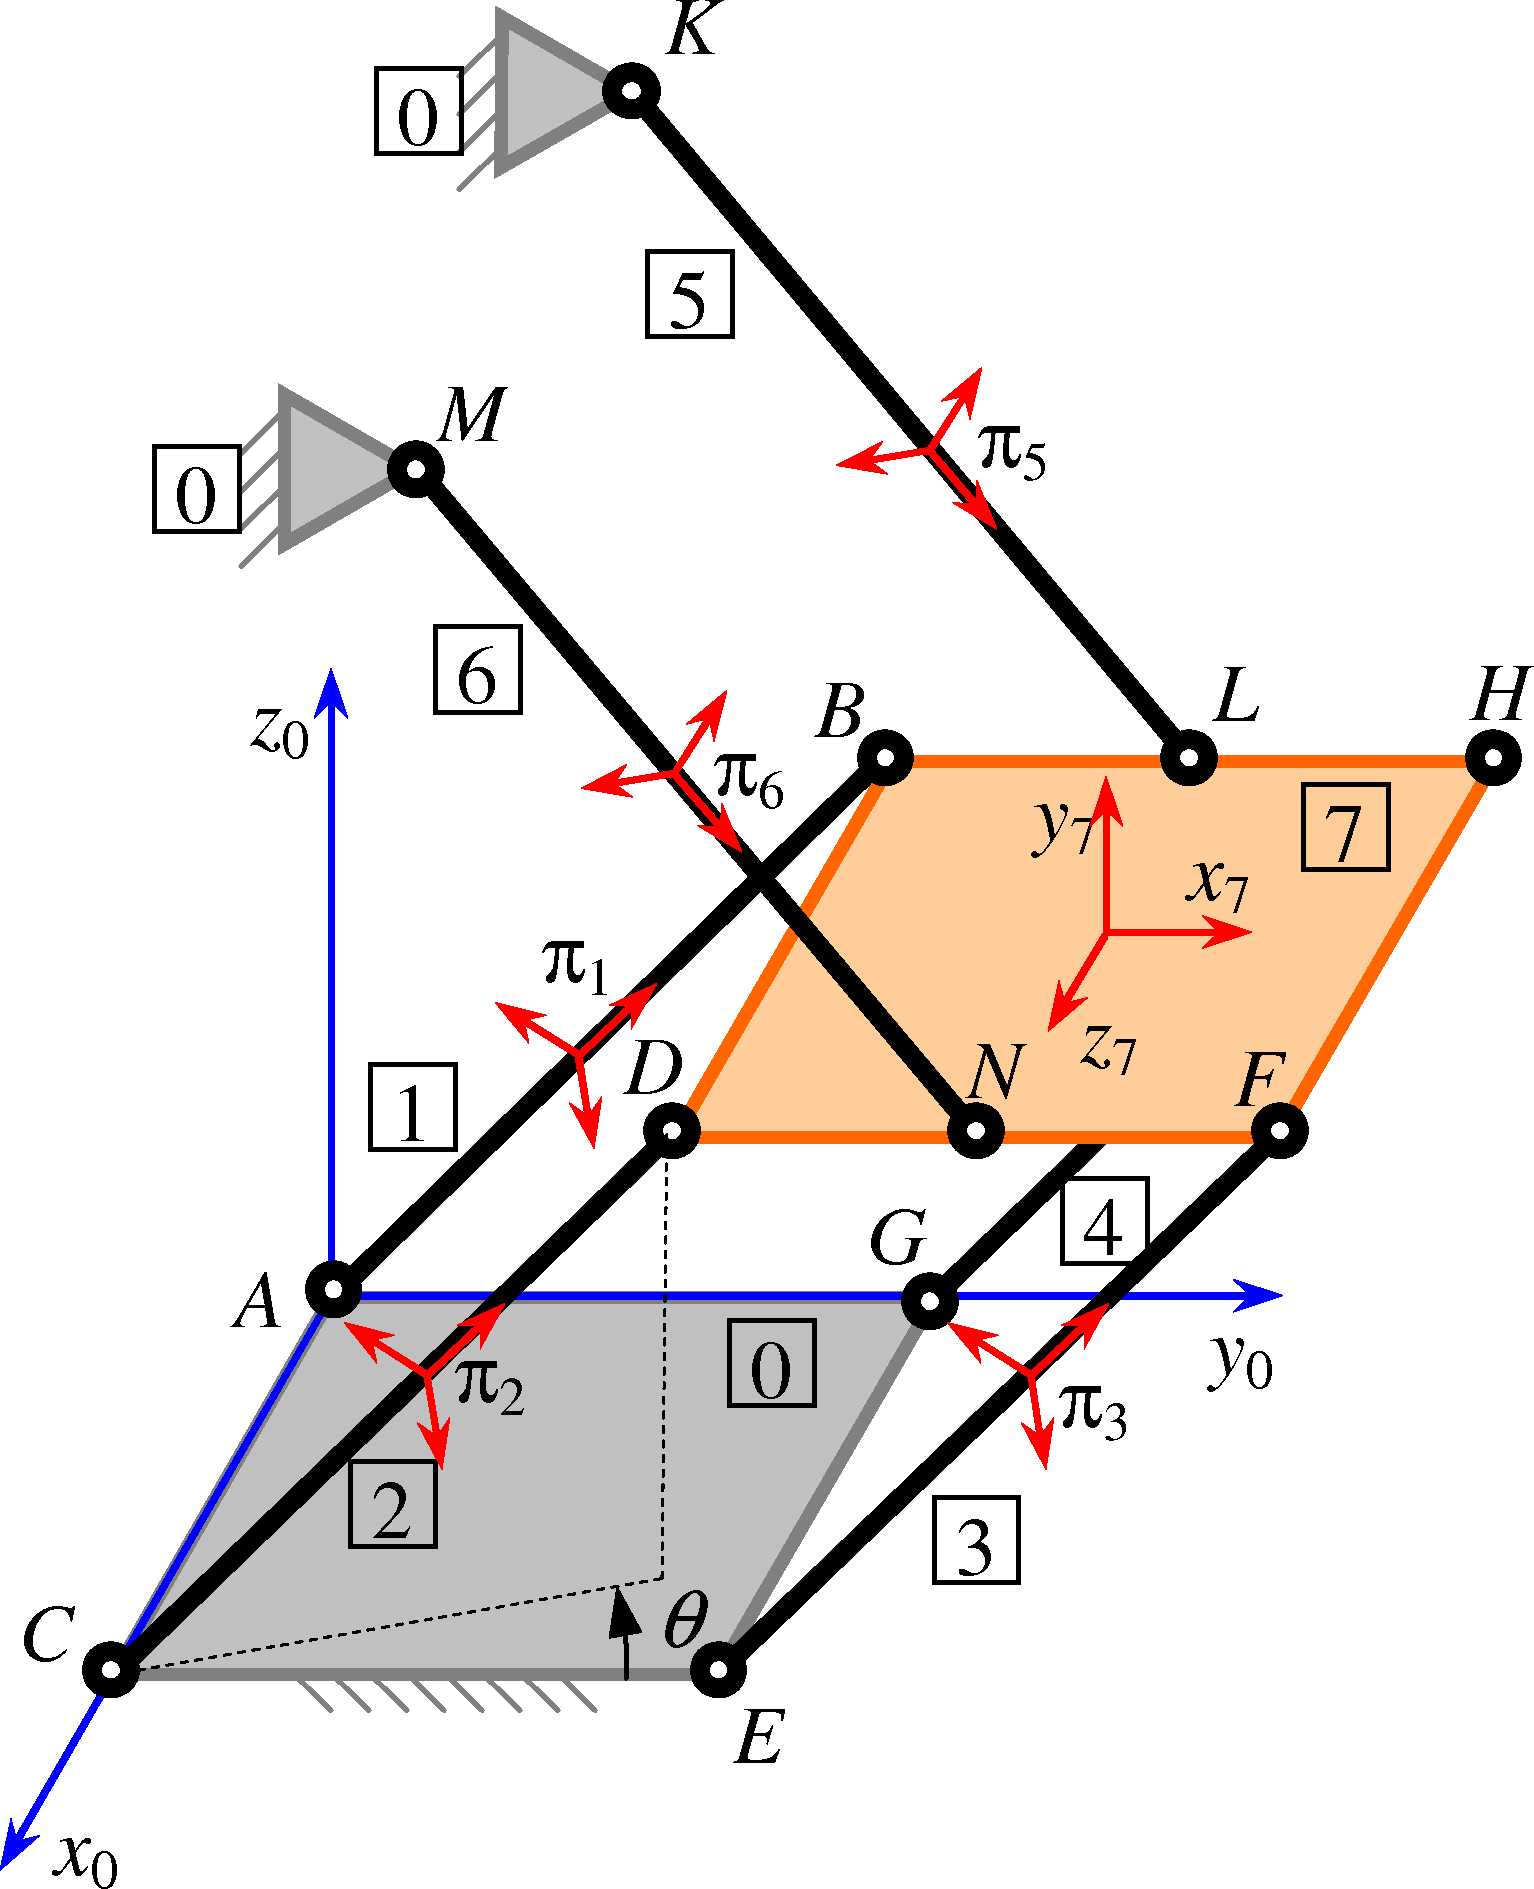
\includegraphics[width=.7\linewidth]{mbs_system.png}
		\captionof{figure}{Multi-body system with 1 DOF}
		\label{fig:mbs}
	\end{minipage}%
	\begin{minipage}{.5\textwidth}
		\centering
		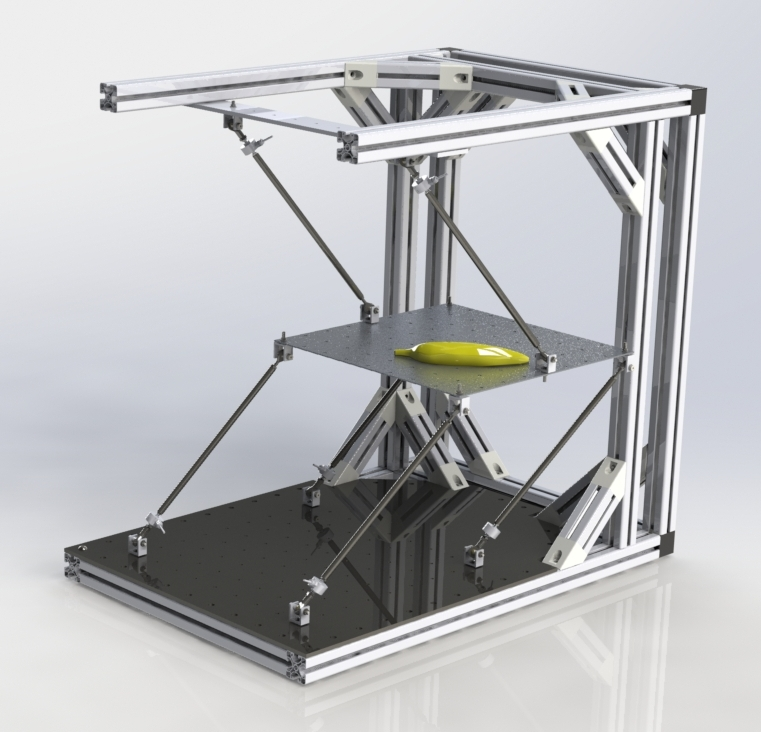
\includegraphics[width=.9\linewidth]{render.jpg}
		\captionof{figure}{Render of MBS}
		\label{fig:render}
	\end{minipage}
\end{figure}

The scientific significance of this mechanism is revealed in the determination of the reaction forces that occur in rods. Mechanism is statically indeterminate which makes it even more difficult to analyze and highlights its research value. The further researches require collecting data from test stand, when the platform moves. State description should contain platform's position and orientation as well as readings from force sensor installed in rods, what is covered by developed system.\\

The mechanism is driven by FANUC M-10iA serial industrial robots. The robot's control system provides arm's tip position. To avoid problems resulting from inaccurate manufacturing the robot is connected to platform center via a drawbar, so the tip's orientation is unusable. Moreover, the position's refresh rate is relatively slow, but can be successfully used in sensor fusion.\\

The mechanism thus presented is a representative example of the application of the developed system. Due to its properties, convetional methods are hard to apply. The proposed solution is challenging as well, but the procedure that lead to working system are structured and split into steps. 

\section{Computer simulation}

